
\documentclass[9pt]{beamer}
%\makeatletter
%\def\beamer@calltheme#1#2#3{%
%	\def\beamer@themelist{#2}
%	\@for\beamer@themename:=\beamer@themelist\do
%	{\usepackage[{#1}]{\beamer@themelocation/#3\beamer@themename}}}
%
%\def\usefolder#1{
%	\def\beamer@themelocation{#1}
%}
%\def\beamer@themelocation{}

%\usefolder{../config}

\usetheme[
block=fill,
titleformat=regular,
progressbar=frametitle
]{metropolis}
%\metroset[everytitleformat=regular] % regular, lowercase, uppercase ]
%\metroset[inner/block=fill]

%\setbeameroption{show notes} 
\usepackage{booktabs}
\usepackage[scale=2]{ccicons}

\usepackage{pgfplots}
\usepgfplotslibrary{dateplot}


%\ Hrvatski znakovi
\usepackage[utf8]{inputenc}
\usepackage[T1]{fontenc}
\usepackage[croatian]{babel}
\usepackage{todonotes}
\usepackage{amsmath}
\usepackage{amsfonts}
\selectlanguage{croatian} % american ngerman
\usepackage{todonotes}

% Koristenje Latin modern fonta
% Bez toga na nekim racunalima baca
% err: Font <taj i taj> at <mala velicina, npr4.0pt> not loadable: Metric (TFM) file not found. \end{frame}
\usepackage{lmodern}


\definecolor{RoyalBlue}{cmyk}{1, 0.50, 0, 0}
%\usepackage{natbib}
%\usepackage{bibentry}
\usepackage{scrextend}
\usepackage{hyperref}
%\usepackage[pdfa=true]{hyperref}
\hypersetup{%
    %draft, % = no hyperlinking at all (useful in b/w printouts)
    %colorlinks=true, 
    linktocpage=true, pdfstartpage=3, pdfstartview=FitV,%
    % uncomment the following line if you want to have black links (e.g., for printing)
    %colorlinks=false, linktocpage=false, pdfborder={0 0 0}, pdfstartpage=3, pdfstartview=FitV,% 
    breaklinks=true, pdfpagemode=UseNone, pageanchor=true, pdfpagemode=UseOutlines,%
    plainpages=false, bookmarksnumbered, bookmarksopen=true, bookmarksopenlevel=1,%
    hypertexnames=true, pdfhighlight=/O,%nesting=true,%frenchlinks,%
    %urlcolor=webbrown, linkcolor=RoyalBlue, citecolor=webgreen, %pagecolor=RoyalBlue,%
    %urlcolor=Blue, linkcolor=Blue, citecolor=Red, %pagecolor=Black,%
    %pdftitle={\myTitle},%
    %pdfauthor={\textcopyright\ \myName, \myUni, \myFaculty},%
    pdfsubject={},%
    pdfkeywords={},%
    pdfcreator={pdfLaTeX},%
    pdfproducer={LaTeX with hyperref and classicthesis}, %
    unicode = true 
} 

%\usepackage[pdftex]{graphicx}
% declare the path(s) where your graphic files are
\graphicspath{{./}{./figures/}}


\newcommand{\executeiffilenewer}[3]{%
	\ifnum\pdfstrcmp{\pdffilemoddate{#1}}%
	{\pdffilemoddate{#2}}>0%
	{\immediate\write18{#3}}\fi%
}
\newcommand{\includesvg}[1]{%
	\executeiffilenewer{#1.svg}{#1.pdf}%
	{inkscape -z -C --file=#1.svg %
		--export-pdf=#1.pdf --export-latex}%
	\input{#1.pdf_tex}%
}


% http://tex.stackexchange.com/questions/83882/how-to-highlight-python-syntax-in-latex-listings-lstinputlistings-command

\usepackage{listings}
\usepackage{color}
\usepackage[semibold]{sourcecodepro}

% Default fixed font does not support bold face
\DeclareFixedFont{\ttb}{T1}{txtt}{bx}{n}{12} % for bold
\DeclareFixedFont{\ttm}{T1}{txtt}{m}{n}{12}  % for normal
% Custom colors
\definecolor{deepblue}{rgb}{0,0,0.5}
\definecolor{deepred}{rgb}{0.6,0,0}
\definecolor{deepgreen}{rgb}{0,0.5,0}


% Python style for highlighting
\newcommand\pythonstyle{\lstset{
		language=Python,
		basicstyle=\small\ttfamily,
		otherkeywords={self},             % Add keywords here
		keywordstyle=\small\ttfamily\color{deepblue},
		emph={MyClass,__init__},          % Custom highlighting
		emphstyle=\small\ttfamily\color{deepred},    % Custom highlighting style
		stringstyle=\color{deepgreen},
		frame=tb,                         % Any extra options here
		showstringspaces=false            % 
	}}
	
	
	% Python environment
	\lstnewenvironment{python}[1][]
	{
		\pythonstyle
		\lstset{#1}
	}
	{}
	
	% Python for external files
	\newcommand\pythonexternal[2][]{{
			\pythonstyle
			\lstinputlisting[#1]{#2}}}
	
	% Python for inline
	\newcommand\pythoninline[1]{{\pythonstyle\lstinline!#1!}}
%\documentclass[ucs]{beamer}
%\usetheme[menuwidth={0.3\paperwidth}]{erlangen}
%\setbeamercovered{transparent=20} 

\usepackage{amsmath,amsfonts,amsthm,amssymb}
\usepackage{setspace}
\usepackage{Tabbing}
\usepackage{fancyhdr}
\usepackage{lastpage}
\usepackage{extramarks}
\usepackage{chngpage}
\usepackage{soul,color}
\usepackage{graphicx,float,wrapfig}
\usepackage{xcolor}
\usepackage[normalem]{ulem}
\usepackage{mathtools}

\definecolor{erlangenlyellow}{RGB}{123, 25, 121}
%\usepackage[utf8x]{inputenc}
%\usepackage{default}
%\usepackage[T1]{fontenc}

\usepackage{verbatim}
\usepackage{listings}


\usepackage{subcaption}
\usepackage{lmodern}

\title{Osnove}

\subtitle{The language of matter writ large}
\institute{Računalna grafika}


\begin{document}
\begin{frame}
 \titlepage
\end{frame}

%\begin{frame}{Sadržaj}
%  \tableofcontents
%  % You might wish to add the option [pausesections]
%\end{frame}
\section{Točka i vektor}
\begin{frame}{Točka}
	\begin{center}
		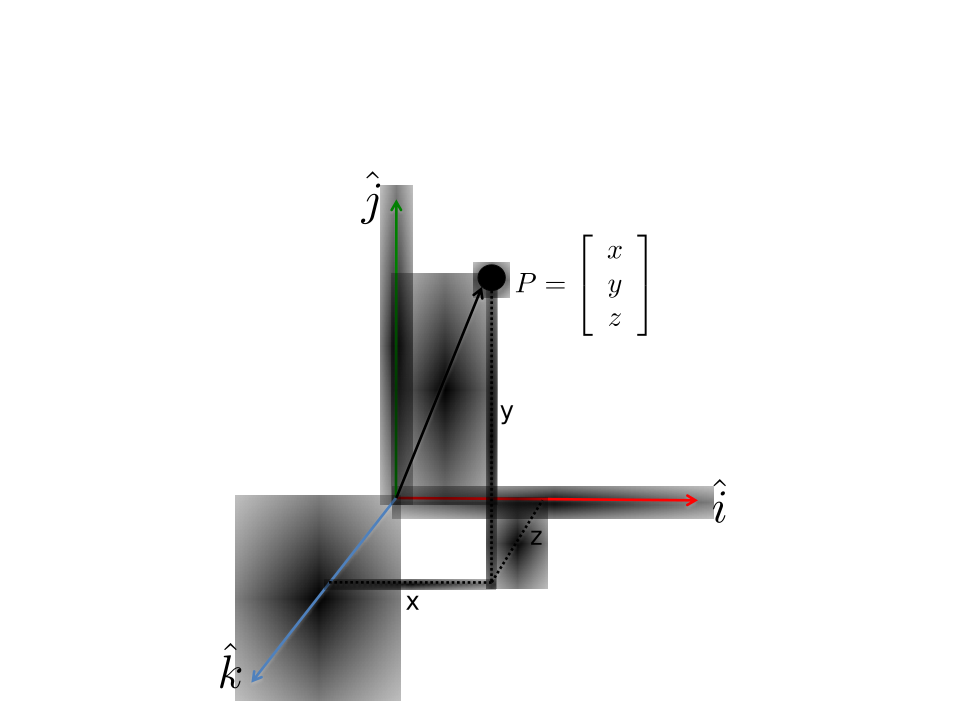
\includegraphics[height=7cm]{./slike/linear_algebra_a_point.png}
	\end{center}
\end{frame}
\begin{frame}{Vektor}
	\begin{center}
		\includegraphics[height=7cm]{./slike/linear_algebra_a_vector.png}
	\end{center}
\end{frame}

\begin{frame}{Točka vs. vektor}
	\begin{itemize}
		\item Točka: \textit{položaj}, ili \textit{pozicija}
		\item Vektor: usmjerena \textit{dužina}. Sastoji se od \textit{smjera} i \textit{duljine} 
		\item isti oblik $\begin{pmatrix} x & y & z\end{pmatrix}^T$ 
		\item homogene koordinate:
		\begin{itemize}
			\item Točka: $\begin{pmatrix} x & y & z & 1\end{pmatrix}^T$
			\item Vektor: $\begin{pmatrix} x & y & z & 0\end{pmatrix}^T$
		\end{itemize}
	\end{itemize}
\end{frame}

\begin{frame}{točka + vektor = točka}
	\begin{center}
		\includegraphics[height=5cm]{./slike/linear_algebra_point_plus_vector.png}
	\end{center}
\end{frame}

\begin{frame}{točka - točka = vektor}
	\begin{center}
		\includegraphics[height=5cm]{./slike/linear_algebra_point_minus_vector.png}
	\end{center}
\end{frame}

\begin{frame}{vektor + vektor = vektor}
	\begin{center}
		\includegraphics[height=5cm]{./slike/linear_algebra_vector_plus_vector.png}
	\end{center}
\end{frame}

\begin{frame}{Vektori: množenje skalarom}
	\begin{center}
		\includegraphics[height=5cm]{./slike/linear_algebra_vector_operations.png}
	\end{center}
\end{frame}

\begin{frame}{Vektori, osnove}
	\begin{align*}
	\vec{u} + (\vec{v} + \vec{w}) &= (\vec{u} + \vec{v}) + \vec{w} \\
	\vec{v} + \vec{w} &= \vec{w} + \vec{v}
	\end{align*}
	\begin{columns}[t]
		\begin{column}{0.4\textwidth}
			\begin{align*}
			a(\vec{v} + \vec{w}) &= a\vec{v} + a\vec{w} \\
			(a+b)\vec{v}  &= a\vec{v} + b\vec{v} \\
			a(b\vec{v})  &= (ab)\vec{v}
			\end{align*}
		\end{column}
	\begin{column}{0.4\textwidth}
		\begin{align*}
		\vec{v} + 0 &= \vec{v}\\
		\vec{v} + \vec{w} &= 0 \rightarrow \vec{w} = -\vec{v} \\
		1\vec{v} &= \vec{v}\\
		\end{align*}
	\end{column}
	\end{columns}
	\begin{align*}
		\vec{v} - \vec{w} &= \vec{v} + (-\vec{w}) \\
		\frac{\vec{v}}{a} &= \left(\frac{1}{a}\right)\vec{v}
	\end{align*}
\end{frame}
\begin{frame}{vektori, još operacija}
	\begin{align*}
	\vec{v}_1 = \begin{pmatrix}
	x_1 \\ y_1 \\ z_1
	\end{pmatrix}
	, \;\;\;
	\vec{v}_2 = \begin{pmatrix}
	x_2 \\ y_2 \\ z_2
	\end{pmatrix}
	\end{align*}
	\begin{itemize}
		\item Skalarni produkt: $\vec{v}_1 \cdot \vec{v}_2 = x_1x_2 + y_1y_2+z_1z_2 = \vec{v}_1^T \vec{v}_2$
		\item Norma (dužina): $\lVert\vec{v}_1 \rVert = \sqrt{\vec{v}_1 \cdot \vec{v}_1} = \sqrt{x_1^2 + y_1^2+z_1^2}$
		\item Normalizacija: $\hat{v}_1 = \frac{\vec{v}_1}{\lVert\vec{v}_1 \rVert} \Rightarrow\hat{v}_1 = 1 $
	\end{itemize}

	\begin{block}{Svojstva skalarnog produkta}
		\begin{itemize}
			\item komutativnost: $\vec{v}_1 \cdot \vec{v}_2 = \vec{v}_2 \cdot \vec{v}_1$
			\item asocijativnost: $\vec{v}_1 \cdot (\vec{v}_2 + \vec{v}_3) = \vec{v}_1 \cdot \vec{v}_2 + \vec{v}_1 \cdot \vec{v}_3$
		\end{itemize}
	\end{block}

\end{frame}

\begin{frame}{vektori i kutevi}
	\begin{itemize}
		\item Kut između dva vektora:
	\end{itemize}
	\begin{center}
		\includegraphics[height=2cm]{./slike/linear_algebra_vector_angle.png}
	\end{center}
	\begin{itemize}
		\item Okomiti vektori
	\end{itemize}
	\begin{center}
		\includegraphics[height=1.5cm]{./slike/linear_algebra_vector_orthogonal.png}
	\end{center}
	Vektori su okomiti ako vrijedi: $\vec{v}_1 \cdot \vec{v}_2 = 0$ \\
	Vektori su \textbf{ortonormalni} ako vrijedi:  $\vec{v}_1 \cdot \vec{v}_2 = 0$, ali $\lVert\vec{v}_1 \rVert = 1$ i $\lVert\vec{v}_2 \rVert = 1$
\end{frame}

\begin{frame}{Vektorski produkt}
	\begin{center}
		\includegraphics[height=3cm]{./slike/linear_algebra_cross_product.png}
	\end{center}
	\begin{align*}
	\vec{v}_1 \times \vec{v}_2 &= \begin{pmatrix}
	\hat{i} & \hat{j} & \hat{k} \\
	x_1 & y_1 & z_1 \\
	x_2 & y_2 & z_2
	\end{pmatrix} \\
	& = \hat{i}(y_1z_2 - y_2z_1) + \hat{j}(x_1z_3 - x_3z_1) + \hat{k}(x_1y_2 - x_2y_1) \\
	& =  \begin{pmatrix}
	y_1z_2 - y_2z_1 \\
	x_1z_3 - x_3z_1 \\
	x_1y_2 - x_2y_1
	\end{pmatrix}
	\end{align*}
\end{frame}

\begin{frame}{Vektorski produkt, svojstva}
	\begin{itemize}
		\item \textbf{nije} komutativan
	\end{itemize}
	\begin{align*}
	\vec{u} \times \vec{v} = -(\vec{v} \times \vec{u})
	\end{align*}
	\begin{itemize}
		\item ali vrijedi distributivnost za zbrajanje i množenje skalarom:
	\end{itemize}
	\begin{align*}
		\vec{u} \times (\vec{v} + \vec{w}) = \vec{u} \times \vec{v} + \vec{u} \times \vec{w} \\
		(a\vec{u}) \times \vec{v} = \vec{u} \times (a\vec{v}) = a (\vec{u} \times \vec{v})
	\end{align*}
\end{frame}

\begin{frame}{Vektorski produkt, norma}
	\begin{center}
		\includegraphics[height=3cm]{./slike/linear_algebra_cross_product_wiki.png}
	\end{center}

	\begin{align*}
	\lVert \vec{a} \times \vec{b} \rVert = \lVert \vec{a} \rVert \cdot \lVert \vec{b} \rVert |\sin \theta|
	\end{align*}
\end{frame}	

\begin{frame}{Pravac}
	\begin{center}
		\includegraphics[height=3cm]{./slike/linear_algebra_pravci.png}
	\end{center}
	\begin{align*}
		P = (E-S)\lambda + S = \vec{v}\lambda + S
	\end{align*}
	\begin{align*}
	\vec{v} = (E-S)
	\end{align*}
	
	\begin{itemize}
		\item $\lambda > 0$: $P$ je \textit{ispred} $S$
		\item $\lambda < 0$: $P$ je \textit{iza} $S$
		\item $\lambda = 0$: $P = S$
		\item $\lambda = 1$: $P = E$
		\item $0 < \lambda < 1$: $P$ je između $S$ i $E$
	\end{itemize}
\end{frame}

\begin{frame}{Udaljenost točke i pravca}
	\begin{center}
		\includegraphics[height=3cm]{./slike/linear_algebra_line_point_distance.png}
	\end{center}
	$\vec{v}_1\cdot \vec{v}_2$ je \textit{projekcija}$\vec{v}_1$ na $\vec{v}_2$!
\end{frame}

\begin{frame}{Udaljenost točke i ravnine}
	Ravnina je zadana točkom $O$ i normalom $\vec{n}$.
	\begin{center}
		\includegraphics[height=6cm]{./slike/linear_algebra_plane_point_distance.png}
	\end{center}
\end{frame}

\section{Baricentrične koordinate}
\begin{frame}{Tri točke}
	\begin{center}
		\includegraphics[height=4cm]{./slike/2d_trokut.png}
	\end{center}
	\begin{itemize}
		\item Trokut je definiran točkama $\mathbf{a}$, $\mathbf{b}$ i $\mathbf{c}$
		\item Definira se koordinatni sustav s baznim vektorima $\mathbf{b} - \mathbf{a}$ i $\mathbf{c} - \mathbf{a}$
		\item Točka se može definirati u tom sustavu s koordinatama (uređeni par) $(\beta, \gamma)$.
		\item Primjer: $\mathbf{p} = (2, 0.5) \rightarrow \mathbf{p} = \mathbf{a} + 2(\mathbf{b} - \mathbf{a}) + 0.5(\mathbf{c} - \mathbf{a}) $
	\end{itemize}
	
\end{frame}
\begin{frame}{Tri točke i trokut, contd.}
	Svaka točka se može definirati kao 
	\begin{align*}
	\mathbf{p} = \mathbf{a} + \beta(\mathbf{b} - \mathbf{a}) + \gamma(\mathbf{c} - \mathbf{a})
	\end{align*}
	Uredimo li malo ovaj izraz:
	\begin{align*}
	\mathbf{p} = (1- \beta - \gamma)\mathbf{a} + \beta\mathbf{b} + \gamma\mathbf{c}
	\end{align*}
	Uvedemo li $\alpha = 1- \beta - \gamma$:
	\begin{align*}
	\mathbf{p} = \alpha\mathbf{a} + \beta\mathbf{b} + \gamma\mathbf{c}
	\end{align*}
	Točka $\mathbf{p}$ se nalazi unutar trokuta ako vrijedi:
	\begin{align*}
	0 \leq \alpha \leq 1 \\
	0 \leq \beta \leq 1 \\
	0 \leq \gamma \leq 1 \\
	\end{align*}
\end{frame}

\begin{frame}{Trokut}
	Obrnuto: Za zadanu točku  $\mathbf{p}$, koliki su $\alpha$, $\beta$ i  $\gamma$?
	\begin{center}
		\includegraphics[height=3cm]{./slike/2d_trokut_01.png}
	\end{center}
	Površina trokuta: 
	\begin{align*}
	A = \frac{1}{2}\lVert (\mathbf{b} - \mathbf{a}) \times (\mathbf{c} - \mathbf{a})\rVert
	\end{align*}
	Također vrijedi: $A = A_a + A_b + A_c$ \\
	
	\begin{block}{Nezgodno}
		Površina trokuta nema predznak, čime se onda \textbf{ne mogu} odrediti $\alpha$, $\beta$ i  $\gamma$
	\end{block}
\end{frame}

\begin{frame}{Trokut, contd.}
	\begin{center}
		\includegraphics[height=3cm]{./slike/2d_trokut_02.png}
	\end{center}
\begin{columns}[t]
	\begin{column}{0.45 \textwidth}
		Možemo odrediti normale:
		\begin{align*}
		\mathbf{n} & = (\mathbf{b} - \mathbf{a}) \times (\mathbf{c} - \mathbf{a}) \\
		\mathbf{n}_a & = (\mathbf{c} - \mathbf{b}) \times (\mathbf{p} - \mathbf{b}) \\
		\mathbf{n}_b & = (\mathbf{a} - \mathbf{c}) \times (\mathbf{p} - \mathbf{c}) \\
		\mathbf{n}_c & = (\mathbf{b} - \mathbf{a}) \times (\mathbf{p} - \mathbf{a})
		\end{align*}
	\end{column}
\begin{column}{0.45 \textwidth}
	Sada je lako:
	\begin{align*}
		\alpha & = \frac{\mathbf{n} \cdot \mathbf{n}_a}{\lVert \mathbf{n} \rVert ^2} \\
		\beta & = \frac{\mathbf{n} \cdot \mathbf{n}_b}{\lVert \mathbf{n} \rVert ^2} \\
		\gamma & = \frac{\mathbf{n} \cdot \mathbf{n}_c}{\lVert \mathbf{n} \rVert ^2}
	\end{align*}
\end{column}
\end{columns}
\end{frame}

\section{Sjecišta}
\begin{frame}{Sjecište pravca i ravnine}
	\begin{center}
		\includegraphics[height=4cm]{./slike/sjeciste_ravnina_pravac_01.png}
	\end{center}
	Pravac: $\textbf{p}(t) = \textbf{e}+t\textbf{D}$
	\\Ravnina: točka na ravnini: $\textbf{p}_0 = (x_0, y_0, z_0)$, normala: $\textbf{n}$
	\\Ako je točka na ravnini:\\
	$(\textbf{p} - \textbf{p}_0)\textbf{n}=0$
	ili:
	$(\textbf{e} +t\textbf{D}- \textbf{p}_0)\textbf{n}=0$
	\\Rješenje: 
	\begin{align*}
	t = \frac{(\textbf{p}_0-\textbf{e})\cdot\textbf{n}}{\textbf{D}\cdot\textbf{n}}
	\end{align*}
\end{frame}

\begin{frame}{Sjecište zrake i ravnine, contd.}
	Može i drukčije: Ako definiramo tri točke na ravnini, $\mathbf{a}, \mathbf{b}, \mathbf{c}$ 
	\begin{center}
		\includegraphics[height=4cm]{./slike/sjeciste_ravnina_pravac_02.png}
	\end{center}
	Točka na ravnini je zadana sa 
	$\textbf{p}(\beta, \gamma) = \textbf{a} + \beta(\textbf{b}-\textbf{a}) + \gamma(\textbf{c}-\textbf{a})$
\end{frame}	

\begin{frame}{Sjecište zrake i ravnine, contd.}
	$\textbf{p}(\beta, \gamma) = \textbf{a} + \beta(\textbf{b}-\textbf{a}) + \gamma(\textbf{c}-\textbf{a})$ 
	\\
	Ako je zadana zraka sa: $\textbf{p}(t) = \textbf{e}+t\textbf{D}$
	$$\textbf{e}+t\textbf{D} = \textbf{a} + \beta(\textbf{b}-\textbf{a}) + \gamma(\textbf{c}-\textbf{a})$$
	Dobije se sustav jednadžbi:
	\begin{align*}
	x_e+tx_D = x_a + \beta(x_b-x_a) + \gamma(x_c-x_a)\\
	y_e+ty_D = y_a + \beta(y_b-y_a) + \gamma(y_c-y_a)\\
	z_e+tz_D = z_a + \beta(z_b-z_a) + \gamma(z_c-z_a)
	\end{align*}
	Nepoznanice su $t$, $\beta$ i $\gamma$
\end{frame}	

\begin{frame}{Sjecište zrake i ravnine, contd.}
	Nakon sređivanja prethodnog izraza:
	\begin{align*}
	(x_a-x_b)\beta + (x_a-x_c)\gamma + x_Dt=x_a-x_e\\
	(y_a-y_b)\beta + (ya-y_c)\gamma + y_Dt=y_a-y_e\\
	(z_a-z_b)\beta + (za-z_c)\gamma + z_Dt=z_a-z_e
	\end{align*}
	Odnosno:
	
	\begin{align*}
	\left[
	\begin{array}{ccc}
	x_a-x_b&  x_a-x_c&  x_D \\ 
	y_a-y_b&  y_a-y_c&  y_D  \\ 
	z_a-z_b&  z_a-z_c&  z_D
	\end{array} 
	\right]
	\left[
	\begin{array}{c}
	\beta \\ \gamma \\ t
	\end{array} 
	\right] =
	\left[
	\begin{array}{c}
	x_a-x_e \\ y_a-y_e \\ z_a-z_e
	\end{array} 
	\right]
	\end{align*}
\end{frame}	

\begin{frame}{Sjecište zrake i ravnine, contd.}
	Još jednostavnije:
	\begin{align*}
	\textbf{A}
	\left[
	\begin{array}{c}
	\beta \\ \gamma \\ t
	\end{array} 
	\right] =
	\left[
	\begin{array}{c}
	x_a-x_e \\ y_a-y_e \\ z_a-z_e
	\end{array} 
	\right]
	\end{align*}
	Zašto $\beta$ i $\gamma$?
\end{frame}

\begin{frame}{Sjecište zrake i ravnine, contd.}
	Ravnina je zadana trima točkama $(A, B, C)$, ili pripadajućim vektorima $\mathbf{a}, \mathbf{b}, \mathbf{c}$.\\
	Svaka točka $\mathbf{P}$ na ravnini se može zapisati kao  $\mathbf{P}(\alpha, \beta, \gamma) = \alpha\mathbf{a} + \beta\mathbf{b}+\gamma\mathbf{c}$, gdje je $\alpha + \beta +\gamma =1$
%	\begin{center}
%		\includegraphics[width=5cm]{slike/ray_trokut_01.png}
%	\end{center}
	Možemo izraziti $\alpha$ i drugačije: $\alpha = 1- \beta - \gamma$ \\
	$\mathbf{P}(\beta, \gamma) = (1- \beta - \gamma)\mathbf{a} + \beta\mathbf{b}+\gamma\mathbf{c} = \mathbf{a} + \beta(\mathbf{b}-\mathbf{a}) + \gamma(\mathbf{c}-\mathbf{a})$\\
	Dakle, izračunamo $t$, $\beta$ i $\gamma$ (pogledati slajdove iznad), onda dobijemo $\alpha$. \\
	Ako vrijedi $\alpha + \beta +\gamma =1$, onda je točka na ravnini.
\end{frame}
\plain{Pitanja?}
\end{document}